% Custom TeX preamble

% Use the article class from KOMA-script
\documentclass[numbers=noenddot,      % Don't suffix numbers with a period
               abstract,              % "Abstract" title
               captions=tableheading, % Table captions go above
               DIV=8]                 % Increase the margin width slightly
              {scrartcl}

% Drag LaTeX into the 21st century
\usepackage[T1]{fontenc}
\usepackage[utf8]{inputenc}

% Enable the micro-typographic functionality of pdfLaTeX
\usepackage[tracking=true,kerning,spacing]{microtype}

% Extra math environments and symbols; this must be loaded before txfonts
\usepackage{amsmath}
\usepackage{units}

% Fonts
\usepackage{txfonts}
\usepackage{inconsolata}

% Set some custom fonts
\setkomafont{pagehead}{\itshape}
\setkomafont{paragraph}{\small\bfseries\sffamily}
\setkomafont{descriptionlabel}{\small\bfseries\sffamily}

% Symbolic footnotes
\renewcommand{\thefootnote}{\fnsymbol{footnote}}

% Caption formatting; we want captions to be delimited by periods as
% opposed to colons
\usepackage{caption}
\captionsetup{labelsep=period}

% Headers and footers
\usepackage{scrpage2}
\pagestyle{scrheadings}

% Tables
\usepackage{booktabs}
\usepackage{eqparbox}
\usepackage{array}
\usepackage{dcolumn}

% Decimal point aligned column
\newcolumntype{d}[1]{D{.}{.}{#1}}

% Padded left aligned column; flush left w/indent; widest centred
\newsavebox{\tempbox}
\newcolumntype{Q}[1]{>{\begin{lrbox}{\tempbox}}
    {c}<{\end{lrbox}\eqparbox{#1}{\unhcopy\tempbox}}}

% Small, mono-space column
\newcolumntype{t}{>{\small\ttfamily}{l}}

% Common \multicolumn (useful for headings &c)
\newcommand{\ccol}[1]{\multicolumn{1}{c}{#1}}
\newcommand{\lcol}[1]{\multicolumn{1}{l}{#1}}

% Figures and graphics
\usepackage[pdftex]{graphicx}
\usepackage{subfig}
\usepackage{tikz}
\usetikzlibrary{calc,trees,positioning,arrows,chains,shapes.geometric,%
    shapes,shadows,matrix}

% Colours; used sparingly of-course
\usepackage{color}
\definecolor{theblue}{rgb}{0.02,0.04,0.58}
\definecolor{thered}{rgb}{0.65,0.04,0.07}
\definecolor{thegreen}{rgb}{0.06,0.44,0.08}
\definecolor{thegrey}{gray}{0.5}

% Code listings
\usepackage{listings}
\lstloadlanguages{C++,[x86masm]Assembler}
\lstset{basicstyle=\scriptsize\ttfamily,
	language=c++,
        keywordstyle=\color{thegreen},
	commentstyle=\color{thegrey},
        stringstyle=\color{thered},
	showstringspaces=false,
	tabsize=4,
	numbers=left,
        numberstyle=\ttfamily,
	stepnumber=1,
	frame=none,
	xleftmargin=3.4pt,
	xrightmargin=3.4pt,
        belowcaptionskip=\medskipamount}

% References and bibliography
\usepackage[round]{natbib}
\bibliographystyle{plainnat}

\renewcommand{\bibfont}{\small}
\renewcommand{\bibsection}{\section*{References\footnote{Local copies of all presentations and papers cited are maintained by the author and available on request.}}}

% PDF specific features
\usepackage[unicode=true, 
            bookmarks=true,
            bookmarksnumbered=false,
            bookmarksopen=false,
            breaklinks=true,
            pdfborder={0 0 1},
            backref=false,
            colorlinks=true,
            linkcolor=black,
            urlcolor=theblue,
            citecolor=theblue,
            hyperfootnotes=false]
           {hyperref}
\hypersetup{pdftitle={Memory Forensics over the IEEE 1394 Interface},
            pdfauthor={Freddie Witherden}}

% Mail-to
\newcommand{\mailto}[1]{\texttt{\href{mailto:#1}{#1}}}

\begin{document}

\title{Memory Forensics over the IEEE 1394 Interface}
\date{\today\footnote{Permanent ID of this document: c1c615827b7647933e5a3d00668d6183}}
\author{Freddie Witherden\footnote{E-mail: \mailto{freddie@witherden.org}}}
\maketitle

\begin{abstract}
  The IEEE 1394 ``FireWire'' interface provides a means for acquiring
  direct memory access.  We discuss how this can be used to perform live
  memory forensics on a target system. We also present
  \emph{libforensic1394} an open-source software library designed
  especially for this purpose. Passive and active applications of live
  memory forensics are analysed. Memory imaging techniques are discussed
  at length. It is demonstrated how the interface can be used both to
  dump the memory of a live system and to compromise contemporary
  operating systems.
\end{abstract}

\section{Introduction}
\label{sec:introduction}

The IEEE 1394 interface is a serial expansion bus found on many personal
computers. Also known under the brand names of \emph{FireWire} by Apple
Inc. and \emph{i.LINK} by Sony it is a means of connecting high-speed
peripheral devices, such as digital camcorders and hard disks, to a
computer. The bus, being peer-to-peer in nature, can also be used to
connect two or more computers together to form an ad-hoc personal
network. One distinguishing feature of the bus---that separates it from
competing interfaces such as the \emph{Universal Serial Bus}---is that
it contains provisions allowing for one device on the bus to directly
read/write from the physical memory of another.

In this paper we show how this feature can be used to perform live
memory forensics on a target system and describe several potential
applications.  As we emphasise in Section \ref{sec:previouswork} the use
of the IEEE 1394 interface for memory forensics is not a new concept
with there being an extensive body of research available. Hence it is
important to stress that the scope of this paper is more evolutionary
than revolutionary.

\paragraph{Roadmap}
In Section \ref{sec:anatomy} we describe how the various parts of an
implementation of IEEE 1394 interact with each other and how these work
together to allow for direct memory access. We elaborate on the
requirement for an SBP-2 unit directory to be present in order for
physical memory access requests to succeed. We discuss how, under the
right circumstances, it is possible to address more than \unit[4]{GiB}
of physical memory through the optional \verb:PhysicalUpperBound:
register.

In Section \ref{sec:libforensic1394}, we present libforensic1394: a
cross-platform library designed especially for the purpose of performing
memory forensics over the IEEE 1394 interface. Unlike existing
libraries, with limited compatibility for modern operating systems,
libforensic1394 supports a wide variety of host/target systems.

Applications, both \emph{passive} and \emph{active}, are discussed in
Sections \ref{sec:passiveapp} and \ref{sec:activeapp}
respectively. Whereas passive applications involve only reading the
memory of a target system, active applications also include writing to
it. In Section \ref{sec:passiveapp} IEEE 1394 based memory acquisition
is discussed within the context of obtaining a reliable and consistent
memory dump of a target system. Hardware based techniques are compared
to software alternatives. Further applications beyond memory acquisition
are discussed in Section \ref{sec:activeapp}. Signature-based code
injection is presented as a means to patch a running binary and used to
bypass the password validation functions on 32- and 64-bit versions of
Microsoft Windows and on recent versions of Apple's Mac OS X operating
system. Techniques for extracting the logon password for a Mac OS X user
are also discussed.

In Section \ref{sec:mitigation} we suggest a variety of mitigation
techniques and comment on their effectiveness.
 
\section{Previous Work}
\label{sec:previouswork}

The direct memory access functionality provided by IEEE 1394 host
controller chips has long been used by system developers to facilitate
\emph{kernel mode debugging}. However the relative obscurity of the bus
outside of Apple computers before 2002 resulted in the issue being
sidelined in lieu of developing techniques for offline
analysis. What follows is a summary of key results heretofore; a more
complete list of which is maintained by \cite{hermann10}.

The first piece of headline-grabbing research came when
\cite{dornseif04} gave a presentation entitled ``Owned by an iPod'' at
PacSec showcasing the profound security implications of direct memory
access. This was followed up by a second presentation ``FireWire --- all
your memory are belong to us'' \citep{dornseif05} at
\mbox{CanSecWest/core05}. These presentations coincided with the release
of \emph{pyfw}---a Python module for interfacing with IEEE 1394
devices. Written atop of the IOKit framework pyfw runs only under Mac OS
X and unfortunately, for reasons to be discussed in Section 3, does not
support targets running Microsoft Windows.

At Ruxcon \cite{boileau06} presented ``Hit by a bus: physical access
attacks with Firewire'' which showed how an appropriately configured
host could be used to gain memory access to a target system running
Windows. The presentation featured a live demonstration of the tool
\emph{winlockpwn} \citep{boileau08} capable of bypassing the password
validation routine in Windows XP SP2. The tool was later released to the
public in early 2008. Shortly after, \cite{panholzer08} from \emph{SEC
  Consult}, confirmed that Windows Vista is also vulnerable to a similar
form of attack. In addition Boileau also released an open-source Python
wrapper around \emph{libraw1394}---a GNU/Linux library for accessing
1394 devices---called \emph{pythonraw1394} that included a suite of
utilities for performing memory dumps. The law enforcement-only utility
\emph{Goldfish} \citep{almansoori09}---capable of extracting the logon
password and open AIM conversions of a Mac OS X
target---appears\footnote{As the author does not have access to the
  utility this assertion is based off of screen captures provided in
  the documentation.} to be a wrapper around these utilities. (See
Section 6 for a discussion on acquiring the logon password under Mac OS
X.)

Another key piece of research is due to \cite{piegdon07} who presents a
variety of techniques for compromising 32-bit GNU/Linux systems using
IEEE 1394. One of the more notable results is the ability to spawn a
shell on the target system using a ``beachhead'' to pipe \verb:stdin:
and \verb:stdout: to the host system. His paper is an invaluable
resource for those interested in analysing GNU/Linux systems. Concrete
implementations were provided as part of the open source \emph{SEAT1394}
suite (which also makes use of libraw1394 for accessing devices).

\cite{halderman08} in their landmark paper on \emph{cold boot attacks}
against encryption keys describe a variety of methods for performing so
called cold boot attacks and on reconstructing AES and RSA keys from a
dump. Cold boot attacks work by leveraging the fact that the contents of
memory modules take a not-insignificant period of time to degrade after
power to a system is cut. The paper presents techniques for extending
this period and using it to \emph{transplant} memory modules between
systems. A viable alternative to IEEE 1394 based access, cold boot
attacks are notable on account of being very difficult to mitigate
through software alone. Hot boot attacks, those which work by rebooting
a system into an alternative operating system, are also discussed.

The Volatility framework \citep{volatility10} is a Python library for
performing forensics on memory dumps of Microsoft Windows systems. It is
capable of extracting artefacts such as the list of running processes.

\section{Anatomy of IEEE 1394}
\label{sec:anatomy}

As was touched on in the introduction, the IEEE 1394 interface is a
peer-to-peer serial expansion bus. Devices on the bus are referred to as
\emph{nodes} with each node being assigned an ID between
$[0..63]$. Consumer grade devices are usually attached to the bus
through one of three connectors:

\begin{description}
\item [6-circuit \emph{alpha}] Found on most personal computers this is
  by far the most common connector and is capable of providing a small
  amount of power to an attached device.
\item [4-circuit \emph{alpha}] Introduced in the 1394a-2000 amendment
  this connector is often found on notebook systems from Sony and
  Hewlett-Packard. Unlike the 6-circuit connector the 4-circuit
  connector lacks ability to provide power to a device. 4-circuit ports
  are much less robust than their 6-circuit counterparts and more prone
  to damage from repeated use.
 \item [9-circuit \emph{beta}] Added in the 1394b-2002 amendment this
   connector is found primarily on high-end Apple computers. Like the
   6-circuit connector it is also capable of providing power to a
   device.
\end{description}

Devices with alpha connectors are usually capable of speeds up to
$\unit[400]{Mbit/s} \simeq \unit[40]{MiB/s}$ (marketed as ``FireWire
400'') while beta connectors are found on ``FireWire 800'' devices
capable of $\unit[800]{Mbit/s} \simeq \unit[80]{MiB/s}$. Backwards
compatibility is built into the standard with heterogeneous and
homogeneous cables being readily available.

Once connected to the bus each node has its own 48-bit address space
which other nodes can make read/write requests to; it is in this manner
that devices on the bus communicate with each other. Every node has a
1024-byte \emph{configuration status ROM\footnote{While termed a ROM it
    can be changed/updated. It is even possible for one device to change
    the ROM of another, although there are few practical applications of
    this.}} (CSR). The purpose of the CSR is to allow a node to
advertise information such as its model/manufacturer and what protocols
it supports; examples of which include the \emph{Serial Bus Protocol}
used by mass storage devices and \emph{IP over 1394}. Support for a
given protocol is indicated by the presence of the relevant \emph{unit
  directory} in the CSR. Operating systems iterate through the list of
unit directories in the CSR to decide how best to handle a newly
inserted 1394 device.

A block diagram showing how applications interact with devices can be
seen in Figure \ref{fig:1394block}, a key part of which is the
\emph{Open Host Controller Interface} \citep{ohci00} chip. The chip,
usually connected over PCI or PCIe, presents the operating system with a
standard interface for interacting with the bus. This has two important
consequences. Firstly that virtually all controller/expansion
cards---irrespective of manufacturer---are supported without the need
for special device drivers. Secondly as support for the standard is so
ubiquitous it is likely that a 1394 port on a personal computer is
backed by an OHCI chip. This makes it feasible \emph{to rely on
  OHCI-specific functionality when analysing the bus}.

\begin{figure}
  \centering
  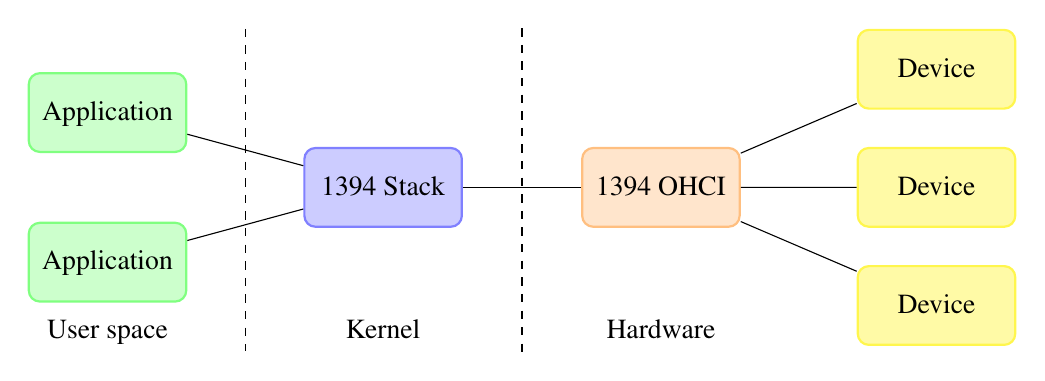
\begin{tikzpicture}[level distance=35mm,node distance=15mm,
                      text height=1.5ex,text depth=0.25ex]

    \begin{scope}[every node/.style={rounded corners,rectangle,thick,minimum width=20mm, minimum height=10mm}]
      \begin{scope}[level 1/.style={sibling distance=19mm,nodes={fill=green!20,draw=green!50}}]
        \node[draw=blue!50,fill=blue!20] (stack) {1394 Stack} [grow=left]
          child {node (app2) {Application}}
          child {node (app1) {Application}};
      \end{scope}

      \begin{scope}[level 1/.style={sibling distance=15mm,nodes={draw=yellow!70,fill=yellow!35}}]
        \node[right=of stack,draw=orange!50,fill=orange!20] (ohci) {1394 OHCI} [grow=right]
          child {node {Device}}
          child {node {Device}}
          child {node {Device}};
      \end{scope}
    \end{scope}

    \node[below=1mm of app1] (userspace) {User space};
    \node at (userspace -| stack) (kernel) {Kernel};
    \node at (userspace -| ohci) (hardware) {Hardware}; 

    \path (app1) -- (stack) node[coordinate,midway] (between1) {};
    \draw (ohci) -- (stack) node[coordinate,midway] (between2) {};

    \draw[dashed] (current bounding box.north -| between1) -- (current bounding box.south -| between1);
    \draw[dashed] (current bounding box.north -| between2) -- (current bounding box.south -| between2);
  \end{tikzpicture}
  \caption{\label{fig:1394block}Simplified block diagram showing how
    1394 devices interact with applications on a personal computer. To
    devices on the bus a 1394 OHCI appears as a device. It is possible
    that some of the attached devices are themselves 1394 OHCI chips.}
\end{figure}

One such piece of functionality of interest to forensics is the
\emph{physical response unit}. Broadly speaking this allows the 1394
OHCI to service read/write requests to certain addresses by treating
them as requests to main memory. Such requests are known as
\emph{physical requests} and are performed by the 1394 OHCI using
\emph{direct memory access} (DMA). As a consequence of this, physical
requests can be handled without any assistance from the system
\citep[][section 3.3]{ohci00}. To be handled by the physical response
unit a request must satisfy several criterion. First that the request
fall within the \emph{low address space} area \citep[][section
1.5]{ohci00}. This is usually defined as being the first \unit[4]{GiB}
of the address space. Secondly the request must be from a node that the
1394 stack has enabled the \verb:PhysicalRequestFilter: for
\citep[][section 5.14.2]{ohci00}.

Although the low address space is usually the first \unit[4]{GiB} of
memory the specification does contain provisions for an \emph{optional}
\verb:PhysicalUpperBound: register that can be used to extend the low
address space above \unit[4]{GiB} \citep[][section
5.15]{ohci00}. Unfortunately, on account of its optional status, very
few OHCI chips include support for it. One notable exception is the
\cite{lsi07} a PCIe 1394b chip found on recent Apple Macintosh computers
and high-end expansion cards which claims to support full 48-bit
physical requests. However, to the author's knowledge no 1394 stacks
take advantage of the \verb:PhysicalUpperBound: register when
present. Hence even with a suitable host controller it is not possible,
without some kind of active intervention, to address more than
\unit[4]{GiB} of memory. The ramifications of this are discussed in
Section \ref{sec:passiveapp}.

The primary purpose of the physical response unit is to save CPU cycles
on the host system. By having the OHCI autonomously process requests it
is possible to both avoid generating an interrupt and an unnecessary
copy of data between the OHCI and main memory. The primary benefactors
of this are protocols which transfer large blocks of data to/from the
host system, such as the \emph{Serial Bus Protocol} (SBP-2). It is
important to emphasise that the use of a physical response unit is not a
requirement for a protocol/device to function but rather a means of
improving performance.

Use of the physical response unit is controlled by the 1394 stack with
per-node granularity. The requirements for a device to be granted access
vary between stacks and are summarised in Table
\ref{tab:physuse}. Looking at the table it is clear that for a device to
be reliably granted use of the unit it must support, or at least claim
to support, the SBP-2 protocol. Indeed this is why the pyfw library
\citep{dornseif04}, described in Section 2, is unable to support target
systems running Microsoft Windows; it does not support adding an SBP-2
unit directory to the CSR of the host system and hence is not given use
of the physical response unit by the target. The newer pythonraw1394
library \citep{boileau06} solves this problem by providing a utility,
\verb:romtool:, to replace the CSR of the host with that of another
device---usually an Apple iPod---which does contain an SBP-2 unit
directory. The limitations of this solution along with less invasive
alternatives are discussed in the next section. Once a host has gained
the use of the physical response unit any read/write requests to the
first \unit[4]{GiB} of the targets address space will be serviced by the
1394 OHCI. This is sufficient for the purposes of performing memory
forensics on a target system.

\begin{table}
  \caption{\label{tab:physuse}Requirements for a device to access
    the physical response unit. Override determines if it is possible to
    restrict use of the unit \emph{without loss of functionality} and is
    covered in Section \ref{sec:mitigation}.}
  \centering
  \catcode`\!=13 \def!{\textcolor{thegreen}{$\bigstar$}}
  \catcode`\_=13 \def_{\textcolor{thered}{$\varnothing$}}
  % Pseudo-footnote; used twice to fix center alignment
  \def\fna{\textsuperscript{\textit{a}}}
  \begin{tabular}{lccc} \toprule
   Stack & Non SBP-2 & SBP-2 & Override \\ \midrule
   Windows XP/Vista & _ & ! & _ \\
   Windows 7 & _ & ! & _ \\
   Mac OS X & ! & ! & ! \\
   Linux old stack & ! & ! & ! \\
   Linux new stack & _ & \phantom{\fna}!\fna & _ \\
   \bottomrule
  \end{tabular}
  \vskip4pt\footnotesize
   ! = available\quad
   _ = not available\quad
  \textit{a}\; requires firewire-sbp2 loaded
\end{table}

\paragraph{Availability}
While not as ubiquitous as the \emph{Universal Serial Bus} (USB) the
IEEE 1394 interface has obtained a reasonable degree of market
penetration and is most often found on higher-end systems. Expansion
cards, however, are readily available in both the PCI and PCIe
interfaces found on desktop systems and the PC Card and ExpressCard
interfaces found on notebooks. The standardised nature of the OHCI means
that such cards seldom require device drivers. The faster 1394b
``FireWire 800'' interface, although uncommon on PCs, is found on
newer/high end Apple Macintosh systems and also on third party expansion
cards, albeit at a higher price point.

The PC Card and ExpressCard interfaces are \emph{hot plug capable}
making it possible to add expansion cards to the system while it is
running. This property is incredibly useful from a forensics standpoint
as it allows a 1394 interface to be added to a system on the fly. Many
operating systems, including Microsoft Windows, Mac OS X and GNU/Linux,
will configure such interfaces automatically \emph{without any
  intervention from the user} and will proceed in doing so even if the
system is locked.

\section{libforensic1394}
\label{sec:libforensic1394}

In order to simplify the process of performing memory forensics over the
IEEE 1394 interface the authors developed \emph{libforensic1394}. The
primary motivation for this was to work around several limitations in
the libraw1394 library---used by pythonraw1394---that prevent it from
being used on modern systems. A GNU/Linux only library, libraw1394 is
designed primarily for use with the old 1394 stack and has only limited
support for the new ``Juju'' stack. Superseded in 2007 with the release
of 2.6.22 the old stack is scheduled for removal in 2.6.37. Since then
many distributions have switched over to using the new stack by default.

A key difference between the two stacks is how changes to the
configuration status ROM are performed. In the old stack it is usual to
\emph{replace} the existing CSR with an entirely new ROM provided by the
application. The change persists until another application flashes its
own CSR. However, this can easily lead to race conditions and issues
regarding unclean termination. In the new stack the problem is solved by
providing an API for \emph{amending} the CSR allowing programs to
\emph{temporarily} add their own unit directories. The new API is both
safer and closer to those provided by the 1394 stacks of other operating
systems. However, a consequence of this change is that any tools which
depend upon the old behaviour---such as \verb:romtool:---no longer
function.

libforensic1394 solves this problem by interfacing with the new stack
directly. As the programming model of the new stack is much closer to
that of other operating systems libforensic1394 is fully supported under
Mac OS X using the IOKit framework. Support for FreeBSD is planned for a
future release. A port to Microsoft Windows is less likely,
however. This is on account of there being no user mode API for
accessing 1394 devices.

\paragraph{Asynchronous requests}
OHCI chips are capable of processing multiple requests in
parallel. Dispatching requests in parallel has the potential to improve
read performance by a factor of three or more. libforensic1394 allows
developers to take advantage of this by providing a \emph{vectorised}
API. Asynchronous interfaces are available on both GNU/Linux and Mac OS
X. However, interfaces are afflicted with serious bugs that can result
in kernel panics when used. libforensic1394 is able to work around some
of these limitations on Mac OS X, albeit at the cost of increased
overhead. Under GNU/Linux the vectorised API falls back to processing
requests synchronously. Due to these limitations performance is
currently suboptimal on both GNU/Linux and Mac OS X.

\paragraph{Benchmarks}
The performance of libforensic1394 is almost entirely determined by the
1394 stack of the \emph{host system} and the OHCI of the \emph{target
  system}. Read requests usually fall into one of two categories:
\emph{block reads}, which involve reading large quantities of sequential
data, and \emph{offset reads}, which involve reading 8--20 bytes out of
every 4096. (Applications of block and offset reads will be discussed in
Sections \ref{sec:passiveapp} and \ref{sec:activeapp} respectively.)
Presented in Table \ref{tab:benchmarks} are benchmarks of
libforensic1394 against several common OHCI chips.

\begin{table}
  \caption{\label{tab:benchmarks}Comparison of block and offset read
    performance for various consumer OHCI chips. Results collected using
    an Apple MacBook running Mac OS X 10.6 with an LSI FW322/323
    ``FireWire 400'' OHCI.}
  \centering
  % Pseudo-footnote
  \def\fna{\textsuperscript{\textit{a}}}
  \begin{tabular}{ld{2.1}d{2.1}d{3.1}d{3.1}} \toprule
    & \multicolumn{2}{c}{Block / \unit{MiB/s}} &
    \multicolumn{2}{c}{Offset / \unit{MiB/s}} \\
    \cmidrule(r{0.3em}){2-3} \cmidrule(l{0.3em}){4-5}
    OHCI & \ccol{Sync} & \ccol{Async} & \ccol{Sync} & \ccol{Async} \\ \midrule
    Creative Labs   &  9.7 & 36.8  & 69.3  & 124.9 \\
    LSI FW322/323   &  9.5 & 31.3  & 69.4  & 110.6 \\
    LSI FW643\fna   & 15.5 & 35.2  & 90.8  & 132.6 \\
    Ricoh R5C832    &  8.2 & 20.2  & 30.0  & 127.3 \\
    Ti TSB43AB22A   &  9.5 & 22.7  & 64.8  & 117.4 \\
    Ti XIO2213A\fna & 10.3 & 35.5  & 31.5  & 128.5 \\
    Via VT6315      &  8.4 & 24.5  & 30.2  & 122.3 \\
   \bottomrule
  \end{tabular}
  \vskip4pt\footnotesize
  \hfil\textit{a}\; IEEE 1394b ``FireWire 800'' controller
\end{table}

It is interesting to note that the Creative Labs OHCI---found on an
Audigy 2 sound card---came closest to saturating the bus. The two 1394b
controllers came second and third respectively, even though they were
limited to 1394a speeds. The performance of two 1394b controllers
connected together is currently unknown. Finally, although the LSI FW322
was only capable of sending data at a rate of \unit[31.3]{MiB/s} it was
capable of receiving it at over \unit[36]{MiB/s}. This appears to be
something of a general trend.

When considering block read performance it is important to leverage the
\emph{maximum request size} supported by the target OHCI. Available from
the CSR of a device, it is usually \unit[2048]{bytes} for 1394a
controllers and \unit[4096]{bytes} for 1394b controllers. Larger
requests entail a lower overall overhead than multiple smaller
requests. This is one of the reasons why the two 1394b controllers
excelled at synchronous reads. In addition to using the largest possible
request size, it is also beneficial to process the resulting data
asynchronously. Any time spent performing actions such as writing the
resulting data to disk is time in which the target OHCI is
idle. Synchronously writing data to disk has the potential to reduce
read performance by a factor of two or more. Solutions to this include
the use of \emph{worker threads} or \emph{memory-mapped files}. The
latter, being a so-called \emph{zero copy} technique, is particularly
attractive from a performance standpoint.

Support for asynchronous requests on GNU/Linux is extremely
temperamental. It is therefore currently not possible to fairly compare
the performance of 1394 stacks. Preliminary results show that while
block read performance is similar to Mac OS X offset read speeds in
excess of \unit[300]{MiB/s} have been observed.

\section{Passive Applications and Software Acquisition}
\label{sec:passiveapp}

Possibly the simplest application of the IEEE 1394 interface in the
context of memory forensics is to \emph{image} the memory of a suspect
system. This can be done by making a series of read requests to the
first few gigabytes of the 1394 address space (which will, in turn, be
handled by the physical response unit of the OHCI, hence, retrieving the
memory contents of the system). However, in order to be useful in a
forensics setting it is necessary that the image be \emph{complete},
\emph{consistent}, \emph{reliable} and leave minimal \emph{tool marks};
terms which are defined more precisely below.

\begin{description}
\item [Complete] Completeness refers to the degree of a system's
  volatile memory contained within an image. This includes not only the
  main memory (DRAM) but also any memory present in expansion cards; as
  of 2010 it is not uncommon for high-end video cards to have in excess
  of \unit[1]{GiB} of dedicated memory. The presence of memory that is
  \emph{paged} or \emph{swapped out} at the time of acquisition is also
  of forensic importance. The definition can also be expanded to include
  the \emph{cache memory} found on central processing units although
  this is usually far less important and hence seldom considered.
\item [Consistent] The memory of a modern computer system is a highly
  dynamic system, constantly changing and being rewritten. Depending on
  the imaging method used, acquiring the memory of a running system can
  take anywhere from a few seconds to a few minutes. During this time it
  is extremely likely that the contents of memory will have
  changed. These changes manifest themselves as \emph{inconsistencies}
  in the resulting image which can be thought of as being analogous to
  the smears found on an overexposed photograph. Such inconsistencies
  severely inhibit forensic analysis.
\item [Reliable] For a memory dump to be reliable it must be free from
  \emph{tampering}, intentional or otherwise. The ways in which software
  running on the system can interfere with the contents of an image are
  discussed later on in this section. Methods which do not depend on
  software running on the suspect system are generally less susceptible,
  or even immune entirely, to tampering. Tampering with an image in a
  surreptitious manner is an extremely difficult task. In addition to
  performing any desired modifications a malicious program must also
  take care to \emph{mask its own presence from the image}. This is an
  incredibly tall order for a piece of software. It is much more likely
  that a program will attempt to perform a \emph{denial of service
    attack} with the objective being to hinder the collection of
  forensic evidence.
\item [Tool marks] The action of plugging a device into a system, say a
  IEEE 1394 cable, or running a piece of software on the system will
  cause the memory contents of the system to change. These undesirable
  changes are known as tool marks. In this paper the definition is
  expanded to also cover any \emph{memory degradation} that might occur
  during the imaging process. Although not an issue for live acquisition
  techniques memory degradation is a limiting factor in cold boot
  methods.
\end{description}

When evaluating an imaging method it is also important to consider any
\emph{prerequisites} that a method might have. For example software
acquisition schemes usually require \emph{root access} on the target
system. It is, more often than not, these prerequisites which limit the
applicability of a method, as opposed to the quality of the resulting
image. Before comparing the relative merits of each acquisition
technique it is first worth outlining what actually constitutes a memory
dump.

\subsection{Address spaces}
\label{sec:addrspace}

All modern processors have the concept of an \emph{address space}. On a
32-bit system this address space is 32-bits in size while on a 64-bit
system it is usually 48-bits in size. This address space is quantised
into \emph{pages} between \unit[4]{KiB} and \unit[4]{MiB} in size. These
pages can then be \emph{mapped}. In the simplest case this mapping is
onto \emph{physical memory} resulting in any reads/writes to the address
space being translated to reads/writes to memory. However, it is also
common to map things other than memory into the address space. The
primary reason for doing this is to allow IO devices to be accessed as
if they were chunks of memory. It is not uncommon for \unit[500]{MiB} of
the address space to be allocated in this fashion. (Incidentally, this
is why a 32-bit system with a $2^{32}=\unit[4]{GiB}$ address space, is
only capable of accessing $\sim$\unit[3.5]{GiB} of memory---the
remainder is used for memory mappings.)

Processes running on a system do not interact with this address space
directly. Instead each process has its own \emph{virtual address space},
presenting it with the illusion that it is the only process
running. Depending on the system there can be between three and four
levels of indirection between the address space of the system and that
of a process. What appears as a contiguous block of memory to a system
is, in reality, a fragmented collection of pages spread throughout the
address space. The specifics of this, and how one can work backwards to
construct the address space of a process, are beyond the scope of this
paper. See \cite{schuster09} and \cite{suiche10} for further details. A
further complication arises from the fact that modern operating systems
make extensive use of \emph{on demand paging}. When demand paging is
used the operating system will only load or \emph{page} data into main
memory when it is required by a program. Moreover, it is also possible
for an operating system to evict unused pages from memory into a
\emph{swap} or \emph{page file}. All of this is completely transparent
to applications and serves to ensure that the system is always making
effective use of available memory, which, until recently, has always
been a highly contested resource. However, because of this it is
possible that elements of an application's virtual address space may not
exist \emph{anywhere} in physical memory.

All of this results in the term \emph{memory dump} being something of a
misnomer; what is actually being dumped is the system's \emph{physical
  address space} which includes not just main memory but also any
mappings which may exist.

\subsection{Imaging methods}
\label{sec:imagingmethods}

Techniques for imaging the memory of a system can be divided up into two
categories: \emph{software based} and \emph{hardware based}. Software
based methods access the memory of a system through executable code
running on the CPU while hardware based methods access it through a
peripheral device attached to the system. As virtually all peripheral
devices use \emph{direct memory access} (DMA) transfers to access memory
hardware based methods are often referred to as being DMA based.

\paragraph{IEEE 1394 and DMA}
Acquisition over the IEEE 1394 interface works by exploiting the
functionality provided by the OHCI physical response unit as described
in Section \ref{sec:anatomy}. As the requests are serviced directly
without any intervention from the CPU 1394 based methods are considered
to be \emph{hardware based}.

The method is particularly attractive from a forensics standpoint as it
only requires commodity hardware. Moreover, as most operating systems
configure 1394 devices automatically upon insertion it can be performed
without the need for administrator privileges on the system and can even
be performed if the system is locked. The hardware nature of the method
serves to greatly reduce the impact of tool marks. However, as stated in
Section \ref{sec:anatomy}, it is usually only possible to image the
first \unit[4]{GiB} of the address space. While this is not currently an
issue, with most consumer systems running 32-bit operating systems, it
is likely to become one in the future. The speed at which memory can be
imaged varies between \unit[20]{MiB/s}--\unit[35]{MiB/s} depending on
the host controller.

Although by far the most common example of hardware based acquisition
others do exist. An example of which is the proof-of-concept Tribble card
\citep{carrier04} a specialist PCI device for imaging the memory of a
running system. While the PCI nature of the Tribble makes it unsuitable
for incident-response it is conceivable that a hot plug capable Express
Card version could be produced. When compared with the IEEE 1394
interface a dedicated card has the advantages of being both faster and
capable of addressing more than \unit[4]{GiB} of memory.

Much of the interest in hardware based methods has been because of the
perceived reliability. However, \cite{rutkowska07} showed how, by using
functionality specific to AMD64 chipsets, it is possible to redirect DMA
requests made by peripheral devices. In doing so she was successfully
able to freeze a system when a device attempted to access a specific
memory address or to cause any such requests to return zeros. A
mechanism to spoof responses to requests was also presented but was
unsupported by the AMD64 chipsets of the time. It is believed that
chipsets by Intel and others possess similar
capabilities. Unfortunately, the presentation is often used as the
primary criticism of IEEE 1394 based techniques. Although valid, its
fringe nature often results in an \emph{overstatement of the reliability
  of the IEEE 1394 interface} which assumes it as being on-par with any
other hardware technique. However, when a read request is made by a
device on the bus to the \emph{low address space} area the OHCI first
checks to see if it should be handled by the physical response unit; if
not the request is forwarded to the 1394 stack for processing. Most
stacks respond to such a request with an error code. However, there is
no reason why a stack---or even an application running on top of the
stack---could not respond with a payload. An application which does just
that under GNU/Linux is presented in Listing \ref{lst:spoof} of Appendix
\ref{sec:listings}.

Analysis of the above application has shown its presence on a system to
be difficult to detect. Despite running in user mode it is capable, when
paired with a suitably fast system, of posting competitive benchmark
results in line with those in Table \ref{tab:benchmarks}. However, if
the precise make and model of the target system's OHCI is known it is
possible to surmise the presence of such an application through
\emph{fingerprinting}. The OHCI physical response unit operates
independently of the target systems CPU. This independence results in
very consistent benchmark results, with an observed standard deviation
of $\pm 2\%$. Any significant deviations from these benchmarks are
likely to be the result of requests being handled by software as opposed
to the physical response unit.

\paragraph{Hibernation file}
Also known as \emph{suspend to disk} hibernation is a feature of many
desktop operating systems which allows for the current state of the
system to be serialised to non-volatile media. This state takes the form
of a \emph{hibernation file} and can be used to resume the system at a
later date. Among other things the hibernation file contains a dump of
any physical memory used by the system. By analysing this file it is
possible to reconstruct portions of the system's address space. To speed
up the hibernation process operating system vendors usually only include
the bare minimum necessary to restore the state of the system. This
means that portions of the address space not currently in use by the
system are omitted. However, these regions can contain useful
information such as the remnants of terminated processes. Hence,
hibernation files do not provide a \emph{complete} image.

Hibernation is often considered as a safer, more reliable, alternative
to \emph{sleep mode} (commonly referred to as \emph{suspend to RAM} or
S3). When a system, traditionally a notebook, is put to sleep all
components other than the memory modules are powered down. As the memory
is still receiving power its contents are preserved, allowing for a
system to reawaken rapidly from suspension. While significantly faster
than hibernation suspension to RAM does require that the memory modules
remain powered for the duration. This is a problem for both desktop and
notebook machines. In an attempt to alleviate this versions of Windows
since Vista and Mac OS X since Leopard have included a feature called
\emph{safe sleep} whereby a hibernation file is created before putting
the system to sleep. In the case of power being cut this file is used to
resume the system. The relevance of this from a forensics standpoint is
that \emph{hibernation files are also present on the machines of users
  who suspend their systems to memory}. This also provides a convenient
means for an investigator to generate a hibernation file. Many systems
are configured to go to sleep when either the power button is pressed
or---in the case of notebooks---when the lid is closed. 

The internal structure of hibernation files varies between operating
systems and is seldom documented. The file is commonly \emph{compressed}
and occasionally \emph{encrypted}. For this reason specialist programs
are required in order to analyse them. In the case of an encrypted
hibernation file the encryption key is often synthesised from the user's
logon password. If the hibernation file was produced when the system was
put to sleep, as is the case with \emph{safe sleep} technologies, the
key can sometimes be retrieved. This is because, in all likelihood,
the key is still resident in the memory of the system and hence can be
obtained using the imaging techniques presented in this section.

The primary advantage of hibernation files is that they are extremely
\emph{consistent}. Indeed, such consistency is necessary in order to
restore the state of a system. In terms of reliability hibernation files
are somewhat questionable. Most operating systems have hooks allowing an
application to be notified when the system is going into
hibernation---making it possible for a malicious application to
obfuscate/terminate itself upon hibernation. This potential is, to an
extent, mitigated by the fact that for a piece of software, malicious or
otherwise, to persist on a system it must be able to survive a
hibernation cycle. Any piece of software incapable of this will have a
decisively short half-life. This places limitations on how an
application can respond to a hibernation. Another potential concern is
that because the file must reside on disk that it can be modified
\emph{ex post facto} by any application with sufficient
privileges. Such a concern can be mitigated by ensuring that no
application on the system has the opportunity to modify the hibernation
file after it has been written. Often this means acquiring the file
before it is used to resume the system. Owing to their very nature
hibernation files can not be used to perform \emph{live analysis} of a
system.

\paragraph{Live software acquisition}
Traditionally, operating systems have provided a special \emph{device
  file} for accessing the physical address space of the system. By
reading from this file an application can produce a memory dump. On
Microsoft Windows the file is specified as \verb:\Device\PhysicalMemory:
while Unix-like systems, including Mac OS X and GNU/Linux, provide
\verb:/dev/mem: for the purpose. Recently, however, there has been a
trend towards limiting access to such files. With the release of Windows
Server 2003 Service Pack 1 Microsoft removed the ability for user mode
applications to access the \verb:PhysicalMemory: device and Apple opted
to disable \verb:/dev/mem: by default with the Intel port of Mac OS X
Tiger. Although \verb:/dev/mem: is still present in many GNU/Linux
distributions it is often limited to the first \unit[1]{MiB} of
memory. Developers of imaging applications have responded to this by
including \emph{kernel modules} to emulate the missing
functionality. Therefore most tools available on the market today are
two-part, consisting of a kernel module to provide an appropriate
devices file and a user mode application to read from this file.

Many imaging tools are available, both open source and
proprietary. Tools for Microsoft Windows include the GPL licensed
\emph{MDD} \citep{mantech09} and the proprietary \emph{MoonSols Windows
  Memory Toolkit} \citep{moonsols10}. For GNU/Linux the \verb:crash:
module \citep{anderson08} can be used to emulate the functionality of
\verb:/dev/mem:. All of these tools require administrator privileges to
run. Whereas Windows and Mac OS X generally maintain \emph{binary
  compatibility} for modules between releases the Linux kernel does
not. It is usually not possible to load a module compiled against one
release of the Linux kernel on a system running a different
release. Investigators wishing to use software acquisition in the field
may therefore be required to keep several versions of a particular
module/driver. The speed of software tools depends heavily on the
bandwidth of the device being used to store/send the image. Using a
\unit[1]{Gbit/s} Ethernet connection or S-ATA hard disk transfer rates
upwards of \unit[80]{MiB/s} can be obtained.

Live software acquisition is plagued by \emph{reliability}
concerns. Imaging tools rely on \emph{system calls} provided by the
operating system in order to function. These calls are required for,
among other things, launching processes, loading modules/drivers into
the kernel and accessing the file system. Any piece of software that can
interfere with these calls has the potential to tamper with the
resulting image. Detection of such software, which may often take the
form of a \emph{rootkit}, is difficult. In some instances it may even be
impossible without the aid of hardware acquisition. This makes live
software acquisition unsuitable for imaging potentially hostile
systems. The use of any software tool will leave behind \emph{tool
  marks}. The extent of these marks is a function of several variables,
including the \emph{memory footprint} of the imaging application, the
size of any kernel modules loaded and the method used to save the
resulting image.  Sending an image to a networked device is likely to
leave fewer marks than writing to a removable mass storage device (which
must itself be inserted into the system).

The two-part design of modern imaging tools is suboptimal insofar as
consistency is concerned. The consistency of an image depends heavily on
the number of active processes running on the system at the time of
acquisition. Processes that are inactive are not modifying memory and so
are unlikely to be the source of inconsistencies. It is therefore
desirable to freeze-out user space applications running on the system
while a memory snapshot is taken. (An approach similar to this is used
in order to hibernate a system.) However, this is only practical if the
imaging tool does not depend on user space in order to function. Herein
lies the problem with current two-part tools in that they all make use
of a user space component. By moving this code into the kernel it
becomes possible to exert a significant degree of control over the
acquisition process. A more in depth discussion on the topic of
consistency in software memory acquisition can be found in
\cite{huebner07}.

\paragraph{Hot boot acquisition}
A crucial result from \cite{halderman08} is that memory takes a
\emph{macroscopic amount of time to degrade} after power is cut. When a
machine is restarted abruptly, say by hitting the reset switch, power is
only lost for a few fractions of a second. It is therefore highly
unlikely that any \emph{degradation} will have occurred. So long as the
BIOS does not erase main memory on start-up its contents will be
available to whatever software is loaded next. Hence, by booting a
system into an \emph{alternative environment} it is possible to produce
a memory image. In their paper \citeauthor{halderman08} present several
such environments suited to the purpose; each making use of a different
attack vector with memory footprints in the region of
\unit[10]{KiB}. Although the contents of main memory are preserved
across a power cycle \emph{memory maps}, in general, are not. This has a
negative impact on the \emph{completeness} of the image.

The environment used for acquisition is independent of the operating
system. This not only improves the \emph{reliability} of the resulting
image but also its \emph{consistency}. Administrator privileges on the
system are also no longer required. However, for the technique to be
applicable there are several constraints which must be satisfied.
Firstly and fore mostly it must be possible to boot the system into an
alternative environment. This may require changing the priority of boot
devices in the BIOS and can be obstructed through the presence of a
\emph{BIOS password}. Furthermore it depends upon the BIOS not clearing
the system memory on start-up. Although this is usually not an issue
many BIOSes provide an option for performing an \emph{extended power-on
  self test} which, when enabled, will perform a destructive memory test
on start-up. In addition \emph{error-correcting code} (ECC) memory,
commonly found in servers, must be initialised to a known state in order
to function correctly. As a consequence it is not possible to perform
hot boot acquisition on systems utilising ECC memory.

While the use of an alternative environment solves the problem of
relying on untrusted \emph{software} it still depends on potentially
untrusted \emph{hardware}. \cite{heasman06} showed that it is possible
to embed rootkits and other malicious code into the BIOSes of
peripherals. Since all environments, including boot loaders and
operating systems, depend on the functionality provided by the BIOS it
is extremely difficult to avoid executing such code. Along with DMA
redirection \citep{rutkowska07} BIOS rootkits are primarily a ``fringe''
concern.

\paragraph{Cold boot acquisition}
When it is not practical to boot the target system into an alternative
environment \emph{cold boot acquisition} can be used. As outlined in
\cite{halderman08} the idea is to \emph{transplant} memory modules from
an untrusted target system to a trusted host system. Hot boot
acquisition can then be performed on the host to obtain a memory
image. This method is applicable whenever a suitable host (memory
recipient) is available and is independent of any software running on
the target.

To transplant memory modules from the target to the host it is necessary
power down both machines. However, as soon as power is cut the contents
of the modules begins to \emph{degrade}. The rate of degradation depends
on both the \emph{speed} and \emph{temperature} of the modules
\citep[][table 2]{halderman08}. Faster modules degrade quicker than
slower modules and cooler modules degrade slower than warmer
modules. Memory modules in a system usually operate at between
$\unit[30]{^\circ C}$ and $\unit[50]{^\circ C}$. At these operating
temperatures the rate of degradation is too high for
transplantation. (Depending on the type of memory and the number of
seconds without power error rates in excess of 40\% can be expected.)
However, by cooling the memory down to $\unit[-50]{^\circ C}$ using
readily available ``canned air'', \citeauthor{halderman08} were able to
dramatically slow down the rate of degradation. At these temperatures
the researchers found that even after a minute without power the error
rate was always below 0.1\%. It is perhaps worth noting that since the
paper was published in 2008 memory speeds have continued to
increase. Further research is required to determine if this observation
still holds with newer modules.

For transplantation to be successful the host and target systems must
use the same type of memory. As of August 2010 desktop systems normally
use either DDR2 or DDR3 while notebook systems normally use SO-DDR2 or
SO-DDR3. A further complication arises if the target system has more
than one memory module. With only a single module present there is only
one possible way of mapping the contents of that module into the
systems' address space. However, when two modules are present there are
potentially four different mappings. In addition to the two \emph{linear
  mappings} there are also two \emph{interleave mappings}. Interleaving,
as depicted in Figure \ref{fig:interleave}, is a means of increasing
memory bandwidth when multiple modules are present. It is available on
most systems since 2005 and generally requires that modules be of equal
capacity and be installed in pairs. The mapping used depends on the
capabilities of the memory controller, the number of memory modules
installed and the physical location of these modules. Should the host
and target systems use different mappings the resulting image will be
jumbled. However, by determining the mappings used by the host/target
systems it is possible to reorder the image. Such determination can be
done post mortem.

\begin{figure}
  \centering
  \newlength\nodewidth
  \setlength\nodewidth{40mm}
  \newlength\nodesep
  \setlength\nodesep{5mm}
  \begin{tikzpicture}[start chain,node distance=\nodesep,
                      b1/.style={fill=red!30,outer sep=0,draw},
                      b2/.style={fill=green!30,outer sep=0,draw},
                      il/.style={minimum width=\nodewidth/6,
                                 minimum height=5mm, outer sep=0,
                                 on chain},
                      il1/.style={il,b1},
                      il2/.style={il,b2}]
    
    \node [b1,minimum width=\nodewidth] (bank1) {Bank 1: \unit[1024]{MiB}};
    \node [b2,minimum width=\nodewidth,right=of bank1] (bank2) {Bank 2: \unit[1024]{MiB}};

    \begin{scope}[node distance=0mm]
      % First two interleave segments
      \node [il1,anchor=north west,xshift=\nodesep/2,yshift=-\nodesep] at
      (bank1.south west) (i1) {};
      \node [il2] (i2) {};
      % Remaining segments
      \foreach \n in {0,1,...,4} {
        \node [il1] {};
        \node [il2] {};
      };
    \end{scope}

    \draw [<->] (i1.south west)
      -- ++(0,-\nodesep*1.5)
      -- ++(\nodewidth*2,0) node[midway,label=below:{\unit[2048]{MiB}},yshift=1.5mm] {}
      -- ++(0,\nodesep*1.5);

    \draw [<->] (i2.south east)
      -- ++(0,-\nodesep/2)
      -- ++(\nodewidth/3,0) node[midway,label=below:{\unit[128]{bits}},yshift=1.5mm] {}
      -- ++(0,\nodesep/2);

  \end{tikzpicture}
  \caption{\label{fig:interleave}Two-way, dual channel memory
    interleaving. Two modules, each connected over a 64 bit bus, are
    presented as a single module with a 128 bit bus. If four modules are
    installed they will be presented as two 128 bit modules. Triple
    channel memory interleaving can also be found on some recent
    systems.}
\end{figure}

\subsection{Summary}
A simplistic comparison of the methods described above can be found in
Table \ref{tab:methcomp}. Looking at the table it is clear that none of
the techniques can be considered perfect in all categories. It is
therefore necessary to choose the most suitable technique on a
case-by-case basis. Often it is advantageous to combine imaging
techniques. Doing so not only increases the chances of successfully
obtaining an image but also makes it more likely that any subterfuge
will be detected. When multiple methods are available it is advisable to
start with the low-risk methods first. For example if 1394 based
acquisition is unsuccessful the worse case scenario is that the target
system becomes unresponsive. Should this occur it is still possible to
\emph{attempt} hot boot acquisition by restarting the
system. Unfortunately the same can not be said of hot/cold boot
acquisition. Should these methods fail there is usually no recourse. For
this reason they are considered by the author to be \emph{methods of
  last resort}.

\begin{table}
  \caption{\label{tab:methcomp}Comparison of memory acquisition methods
    when performed on a desktop/notebook system.}
  \centering
  % Good/Very good/Poor/Very poor/Yes/No defs
  \def\g{\textcolor{thegreen}{$\bigstar$}}
  \def\vg{\textcolor{thegreen}{$\bigstar\bigstar$}}
  \def\b{\textcolor{thered}{$\hskip0.15em\varnothing$}}
  \def\vb{\textcolor{thered}{$\hskip0.15em\varnothing\hskip0.25em\varnothing$}}
  \def\y{\hskip0.15emYes}
  \def\n{\hskip0.15emNo}
  \begin{tabular}{lQ{comp}Q{comp}Q{comp}Q{comp}Q{comp}Q{comp}} \toprule
    & \multicolumn{2}{c}{Hardware} & \multicolumn{4}{c}{Software} \\
    \cmidrule(r{0.3em}){2-3} \cmidrule(l{0.3em}){4-7}
    Characteristic & \ccol{1394} & \ccol{Other} & \ccol{Hiberfile} & \ccol{Live} & \ccol{Hot boot} & \ccol{Cold boot} \\
    \midrule
    Prerequisites & \g  & \vb & \g  & \b  & \g  & \vb \\
    Completeness  & \g  & \vg & \b  & \vg & \b  & \b  \\
    Consistency   & \b  & \b  & \g  & \b  & \vg & \vg \\
    Reliability   & \b  & \g  & \b  & \vb & \g  & \vg \\
    Tool marks    & \g  & \g  & \g  & \vb & \g  & \g  \\
    Degradation   & \vg & \vg & \vg & \vg & \g  & \b  \\
    Risk factor   & \g  & \b  & \vg & \g  & \vb & \vb \\
    In vivo       & \y  & \y  & \n  & \y  & \n  & \n  \\
    \bottomrule
  \end{tabular}
  \vskip4pt\footnotesize
   \vg = very good\quad
   \g = good\quad
   \textcolor{thered}{$\varnothing$} = poor\quad
   \textcolor{thered}{$\varnothing\varnothing$} = very poor
\end{table}

\section{Active Applications}
\label{sec:activeapp}

The OHCI physical response unit is also capable of servicing write
requests to main memory. At first glance use of such functionality
appears to be at odds with the core principles of forensic
science. In this section it will be shown how, when applied
appropriately, so called \emph{active memory forensics} can aid in the
analysis of a system.

In Section \ref{sec:passiveapp} several techniques for imaging the
memory of a system were presented. Although the imaging process may be
performed \emph{in vivo} the analysis of the image is usually performed
\emph{post mortem}. However, the \emph{state} of a modern computer is
increasingly becoming more than the sum of its memory and drive
contents. Some states, such as \emph{network sockets} can not be simply
serialised to disk. Post mortem analysis may be able to \emph{infer}
their existence but can not be used to \emph{interact} with them. This
is where in vivo or live forensics comes into play. For live forensics
to be effective it is necessary to have administrator privileges on the
target system. When analysing a system in a hostile environment the
required credentials might not be available to the investigator. Or,
worse still, it is possible that the system is \emph{locked}, inhibiting
even rudimentary analysis.

Active memory forensics solves this problem by eliminating the need for
such credentials. By overwriting parts of the target operating system it
is possible to obtain unfettered access to the system. In this section
techniques will be presented for bypassing the authentication routines
of Microsoft Windows and Mac OS X. Application of these techniques will
allow an investigator to gain root access to the target system. 

\paragraph{Subverting FDE}
Acquiring unrestricted access to a target system is not just useful when
performing live forensics. Another application is in subverting
\emph{full disk encryption} (FDE). Implementations of FDE such as
\emph{DriveTrust} by \cite{seagate06} work by storing the key in a
write-only register in the drive. The key is requested from the user
when the computer is booted and then purged from memory. All
encryption/decryption is then performed transparently by the drive.

Consider the following scenario in which an IEEE 1394 equipped computer
making use of FDE is locked. Neither classic drive forensics or passive
acquisition are of much use here---the drive is encrypted and the key is
not in memory. Without the cooperation of the owner the situation is at
an impasse. However by leveraging the active capabilities of the 1394
interface it is possible to forcibly unlock the system. Once unlocked
the contents of the drive can be copied, block for block, to an external
medium.

\subsection{Signature matching}
The authentication schemes used by modern operating systems are
incredibly complex. The process of validating a password involves the
calling of many hundreds of functions and the execution of many
thousands of instructions. Through either reverse engineering or
inspection of the source code it is possible to determine which of these
functions are responsible for deciding if an authentication attempt is
successful or not. By short circuiting any one of these functions it is
possible to gain access to the system.

Main memory, as described in Section \ref{sec:addrspace}, is divided up
into \emph{pages}. As the order of these pages is random the contents of
main memory are heavily \emph{fragmented}. It is therefore not possible
to determine in advance in which page a piece of code will reside. Often
the location of a piece of code will change when a system is
rebooted. It is therefore necessary to be able to determine the location
of a function at runtime. Perhaps the simplest means of accomplishing
this is through a technique known as \emph{signature matching}. Using
signature matching it is possible to locate the page and offset of a
function in memory. The idea is to find a piece of code which uniquely
identifies a given function and then use this piece of code as a
\emph{signature}. Each memory page can then be searched for this
signature in order to locate the desired function. Once located the
function can be \emph{patched} and its behaviour altered. For
simplicity, function signatures are usually chosen to contain the pieces
of code which require patching.

\paragraph{Limitations}
Signature matching is not 100\% reliable. As functions are identified
only by a signature---usually between 8--12 bytes---there is always the
possibility of \emph{false positives}. The chances of a signature being
unique increase dramatically should the signature contain one or more
\emph{constants}. Examples of suitable constants include \emph{jump
  offsets}, integer \emph{enumerations} and \emph{memory addresses}. The
impact of false positives can be reduced by doing a complete scan over
the memory image prior to patching. Doing so allows for multiple
instances of a signature in an image to be identified and for any false
positives to be eliminated.

It is possible for a signature to be split between two memory pages. The
probability of such a split depends on the page size and signature
length with
\[
  \Pr(\textrm{split} \mid s,P) = \frac{s-1}{P}
\]
where $s$ is the length of the signature and $P$ is the page size. For a
signature of length 12 bytes and a page size of 4096 bytes
\[
  \Pr(\textrm{split} \mid s=12,P=4096) = \frac{11}{4096} \simeq 0.3\%.
\]

The effect of a signature split is to cause the first $n$ bytes of a
signature to appear at the end of one page and the remaining $s-n$ bytes
to appear at the start of another. When a signature split is suspected
it is often easier to change signatures and gain access to the system
through an alternative attack vector.

\paragraph{Offset matching}
It is generally not possible to predict the precise memory \emph{page}
that a signature will reside in, but, it is possible to predict the
\emph{offset} in the page. This property, illustrated in Figure
\ref{fig:pageoff}, allows signature matching to make use of \emph{offset
  reads}. Compared with sequential block reads offset reads are both
faster and are less likely to yield false positives. However, this comes
at the cost of robustness; any updates to the library/executable have
the potential to change the offset of a signature. Programs should
therefore be prepared to fall back to a linear search should offset
matching fail.

\begin{figure}
  \centering
  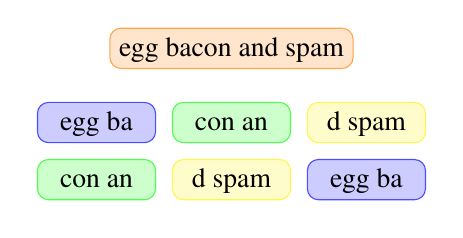
\begin{tikzpicture}
    [node distance=3mm,
     pg/.style={outer sep=0,rounded corners, minimum width=15mm,
                text height=1.5ex,text depth=0.25ex},
     a/.style={pg,fill=blue!20,draw=blue!70},
     b/.style={pg,fill=green!20,draw=green!70},
     c/.style={pg,fill=yellow!20,draw=yellow!70},
     v/.style={pg,fill=orange!20,draw=orange!70}]
    \def\A{\node[a] {egg ba};}
    \def\B{\node[b] {con an};}
    \def\C{\node[c] {d spam};}

    \node[v] (virt) {egg bacon and spam};

    \matrix[row sep=2mm, column sep=2mm,
            matrix anchor=north,below=of virt.south] (phys)
    {
      \A &  \B & \C \\ \B &  \C & \A \\
    };      
  \end{tikzpicture}
  \caption{\label{fig:pageoff}How the phrase ``egg bacon and spam''
    might be ordered in physical memory on a system with a page size of
    six bytes. While the \emph{order} of pages may change the
    \emph{contents} do not. Given the signature ``sp'' it is only
    necessary to check the third and fourth byte of each page for a
    match.}
\end{figure}

\paragraph{Matching programs}
A sample signature matching application can be found in Listing
\ref{lst:patch} of Appendix \ref{sec:listings}. The program is written
in Python and uses libforensic1394. While unsuitable for use in a
production environment it does demonstrate the basic principles behind
signature matching/patching. A more complete program can be found as
part of the Volatility framework \citep{volatility10}.

\subsection{Microsoft Windows}
Authentication on Microsoft Windows is handled by msv1\_0.dll. While the
source code is not available debugging symbols are provided for 32-bit
versions of Windows. Analysis of the library shows many of the functions
to be suitable candidates for short circuiting. The approach taken here
is similar to that of \cite{panholzer08} and focuses primarily on
\verb:MsvpPasswordValidate:. 

\verb:MsvpPasswordValidate: is an internal helper function that uses
\verb:RtlCompareMemory: to compare two password hashes. Disassembly of
the relevant portions can be found in Listing \ref{lst:msvp}. Although
there are many ways to short circuit the function the simplest is to
disable the conditional jump on line seven. This can be done by
replacing it no-operation instructions. The nature of the jump (short or
long) and the address of \verb:$_1: varies between Windows version.
A list of signatures along with their replacements and observed page
offsets can be found in Table \ref{tab:msvpsig}.

\lstinputlisting[float,language={[x86masm]Assembler},caption={\label{lst:msvp}\texttt{MsvpPasswordValidate}
  on a 32-bit system running Windows 7.}]{listings/msvp.asm}


\begin{table}
  \caption{\label{tab:msvpsig}Signatures and known offsets for
    \texttt{MsvpPasswordValidate} in msv1\_0.dll.}
  \centering
  \begin{tabular}{lttl} \toprule
    Windows Version & \lcol{Signature} & \lcol{Patch} & Offset \\ \midrule
    XP SP3 (x86)  & 83F8107511B0018B & 83F810\underline{9090}B0018B &
    2218 \\
    Vista SP1 (x86) & 83F8107513B0018B & 83F810\underline{9090}B0018B &
    1074  \\
    7 (x86) & 83F8107513B0018B & 83F810\underline{9090}B0018B &
     2342 \\
    7 (x64)& C60F85C0B80000B8  & C6\underline{909090909090}B8 & 657 \\
\bottomrule
  \end{tabular}
\end{table}

In order to yield a match the signatures in Table \ref{tab:msvpsig}
depend on the \emph{offset} of \verb:$_1: remaining constant. That is to
say the location of \verb:$_1: relative to the jump site. On 32-bit
versions of Windows this is not a problem; \verb:$_1: is directly
adjacent to the main body of \verb:MsvpPasswordValidate: so unlikely to
change between revisions. However, on 64-bit versions \verb:$_1: is
located some \unit[46]{KiB} away. Any modifications to this intermediate
body of code can potentially cause the offset to change. This results in
the 64-bit signature being far less robust than its 32-bit
counterparts. Indeed, during the development of libforensic1394 the
offset was observed to change from \verb:0xB8A0: to \verb:0xB8C0: as a
result of an update to msv1\_0.dll. One potential solution to this is to
use \emph{fuzzy matching}, treating the jump offset as an unknown
variable. Resilience against false positives can be improved by
increasing the length of the signature and requiring the offset be in
the vicinity of $\unit[46 \pm 5]{KiB}$.

In addition to \verb:MsvpPasswordValidate: there are many other viable
approaches. For example it is possible to short circuit the
\emph{password required} function that determines if a user requires a
logon password or not. This is the technique used by \emph{winlockpwn}
\citep{boileau08}. Another option is to modify \verb:RtlCompareMemory:
to always return 16---the length of a password hash---when comparing
sources of that size.

\subsection{Mac OS X}
The DirectoryServices daemon is tasked with performing authentication
under Mac OS X. As part of Apple's open source offering the C++ source
code is readily available. Analysis of the source shows
the \verb!CDSLocalAuthHelper::DoShadowHashAuth! method to be responsible
for password validation \citep{apple05}.

Mac OS X makes extensive use of \emph{fat binaries}. To be able to
bypass all variants of 10.5 ``Leopard'' and 10.6 ``Snow Leopard'' a
minimum of \emph{four} signatures are required. However, for the sake of
brevity, only the 64-bit Intel case for 10.6 is considered here.

Disassembly of \verb:DoShadowHashAuth: shows the line
\begin{center}
\lstinline[language={[x86masm]Assembler},basicstyle=\small\ttfamily]
{mov r15d, ffffc8f6h}
\end{center}
as being responsible for indicating a failed authentication attempt. By
replacing \verb:0xFFFFC8F6: (defined as \verb:eDSAuthFailed:) with
\verb:0x0: (\verb:eDSNoErr:) it is possible to short circuit the
function.

\begin{table}
  \caption{\label{tab:osxsig}Signatures and known offsets for
    \texttt{DoShadowHashAuth}.}
  \centering
  \begin{tabular}{lttl} \toprule
    OS X Version & \lcol{Signature} & \lcol{Patch} & Offset \\ \midrule
    10.6.4 (Intel 64-bit)  & 41BFF6C8FFFF48C78588 & 41BF\underline{00000000}48C78588 &
    1999 \\
    \bottomrule
  \end{tabular}
\end{table}


\paragraph{Extracting the logon password}
While processing memory dumps from a Mac OS X system the user's logon
password was found to occur several times. This is not a new discovery;
a similar observation was made by \cite{halderman08} and the
law enforcement-only program \emph{Goldfish} \citep{almansoori09} claims
to be able to extract this password from a dump.

The number of password instances was found to vary between 4--10
depending on the configuration of the system. The disk encryption system
\emph{FileVault} was---somewhat ironically---discovered to be
responsible for several of these instances. It is believed that Mac OS X
retains the logon password in memory for use by services such as
\emph{Keychain}. For an instance to be a viable candidate for extraction
the memory \emph{surrounding} it must be uniquely identifiable and
predictable. Only two instances were able to satisfy this constraint on
all platforms. The following regular expression was found to reliably
extract the logon password on both 10.5 ``Leopard'' and 10.6 ``Snow
Leopard''
\begin{center}
  \texttt{managedUser\char`\\x00\{5\}password\char`\\x00\textcolor{theblue}{(.*?)}\char`\\x00shell}
\end{center}
with the password being extracted into the first capture group
(highlighted in blue).

Where applicable password extraction should be preferred over memory
patching techniques; unlike patching password extraction is an entirely
\emph{passive} operation. It is also highly likely that the extracted
password is capable of granting access to other systems and/or services.

\section{Mitigation}
\label{sec:mitigation}

The risk posed by unsecured IEEE 1394 interfaces is not
insignificant. As was alluded to in Table \ref{tab:physuse} many stacks
provide an option to restrict access to the physical response
unit. Depending on the stack this can sometimes be done without
affecting device compatibility.

\begin{description}
\item[Microsoft Windows] No versions of Windows provide control over the
  physical response unit. Without resorting to third-party solutions the
  best option is to disable the 1394 stack entirely before leaving a
  system unattended. This can be done from \emph{Device Manager}.
\item[Mac OS X] Access to the physical response unit can be disabled by
  setting a \emph{firmware password}. This can be done using the
  \emph{Open Firmware Password} utility provided on the Mac OS X install
  DVD. Despite the presence of ``Open Firmware'' in the title it also
  supports EFI-based Intel Macintoshes. Although this effect is
  undocumented by Apple it has been observed under both 10.5 and
  10.6.
\item[GNU/Linux] The old stack provides the module option
  \verb:phys_dma=0: to disable the unit. No such parameter is provided
  by the new ``Juju'' stack. However, it is worth noting that while the
  old stack always allows nodes access to the unit the new stack does so
  on an on-demand basis. Currently only the firewire-sbp2 module
  utilises the unit. Unloading this module will prevent use of the unit
  at the cost of disabling access to 1394 mass storage devices.
\end{description}

It is very difficult to protect a \emph{live} system against an attacker
with \emph{physical access}. While many of the forensic strategies
outlined in Sections \ref{sec:passiveapp} and \ref{sec:activeapp} can be
mitigated against it is the heretofore \emph{unknown} techniques that
pose the real threat. New methods of analysis---both hardware and
software---are continually being developed by researchers in the
field. It is therefore more productive to treat main memory as an
inherently insecure resource. All current and future attacks can be
voided by physically powering a system off when unattended.

\section{Conclusions}
\label{sec:conclusions}

In this paper the IEEE 1394 ``FireWire'' interface was presented within
the context of performing memory forensics. It was shown how the
interface can be used for imaging the memory of a target system. It was
also demonstrated how an attacker could compromise the reliability of
the interface if given access to the target system. The interface was
compared with alternative memory acquisition techniques and was
determined to be ideal for performing live memory forensics.

The case was made for utilising the write capabilities of the interface
to aid in the forensic analysis of a system. Signature matching was
shown to be an effective means of aggressively gaining access to a
system.

\paragraph{Future work}
It is hypothesised that the \emph{Serial ATA} (S-ATA) interface, along
with its external variant eS-ATA, can also be used to acquire DMA to a
target system. S-ATA is a widely deployed, hot-plug capable, interface
for attaching disk drives to a system. Compared with the IEEE 1394
interface S-ATA boasts faster transfer speeds and greater
availability. Further analysis of both the ATA specification and the
capabilities of disk controllers is required to determine the viability
of this approach.

Another aspect worthy of further consideration is that of a kernel-mode
acquisition tool. By moving more of the acquisition process into the
kernel it should be possible to improve the consistency of the image.

\section*{Acknowledgements}
I would like to thank Matt Archer, Mike Auty, Michael Nielsen and Rob
Valkass for their helpful comments, suggestions and
contributions. Without them this paper would not have been possible. In
addition, I would also like to thank Stefan Richter for the assistance
he provided me with during the development of libforensic1394.

\appendix
\newpage
\section{Code Listings}
\label{sec:listings}

\lstinputlisting[caption={\label{lst:spoof}A proof-of-concept GNU/Linux
  application written against the ``Juju'' stack to spoof responses to
  requests made to \emph{low address space}. To function as intended it
  is necessary to first unload the firewire-sbp2
  module.}]{listings/spoof.c}

\newpage
\lstinputlisting[language=Python, caption={\label{lst:patch}A minimal
  signature matching application in Python. It is not recommended for
  production use on account there being no false positive detection or
  linear fall back. Usage is: \texttt{\$ ./patch.py signature patch
    offset}.}]{listings/patch.py}

\newpage
\bibliography{firewire}

\end{document}